\documentclass[10pt,a4paper,twocolumn,twoside]{article}
\usepackage[utf8]{inputenc}
\usepackage[catalan]{babel}
\usepackage{multicol}
\usepackage{graphicx}
\usepackage{fancyhdr}
\usepackage{times}
\usepackage{titlesec}
\usepackage{multirow}
\usepackage{lettrine}
\usepackage[top=2cm, bottom=1.5cm, left=2cm, right=2cm]{geometry}
\usepackage[figurename=Fig.,tablename=TAULA]{caption}
\usepackage{verbatim}
\usepackage{float}
\usepackage{ulem}
\usepackage{pdfpages}

\usepackage[caption=false]{subfig}

\usepackage[toc,page]{appendix}

\captionsetup[table]{textfont=sc}

\author{\LARGE\sffamily Gerard Martínez Espelleta}
\title{\Huge{\sffamily Visualització, creació i millora de terrenys 3D}}
\date{\today}

\newcommand\blfootnote[1]{%
  \begingroup
  \renewcommand\thefootnote{}\footnote{#1}%
  \addtocounter{footnote}{-1}%
  \endgroup
}

%
%\large\bfseries\sffamily
\titleformat{\section}
{\large\sffamily\scshape\bfseries}
{\textbf{\thesection}}{1em}{}

\begin{document}

\fancyhead[LO]{\scriptsize Gerard Martínez Espelleta: Visualització, creació i millora de terrenys 3D}
\fancyhead[RO]{\thepage}
\fancyhead[LE]{\thepage}
\fancyhead[RE]{\scriptsize EE/UAB TFG INFORMÀTICA: Visualització, creació i millora de terrenys 3D}

\fancyfoot[CO,CE]{}

\fancypagestyle{primerapagina}
{
   \fancyhf{}
   \fancyhead[L]{\scriptsize TFG EN ENGINYERIA INFORMÀTICA, ESCOLA D'ENGINYERIA (EE), UNIVERSITAT AUTÒNOMA DE BARCELONA (UAB)}
   \fancyfoot[C]{\scriptsize \today , Escola d'Enginyeria (UAB)}
}

%\lhead{\thepage}
%\chead{}
%\rhead{\tiny EE/UAB TFG INFORMÀTICA: TÍTOL (ABREUJAT SI ÉS MOLT LLARG)}
%\lhead{ EE/UAB \thepage}
%\lfoot{}
%\cfoot{\tiny{February 2015, Escola d'Enginyeria (UAB)}}
%\rfoot{}
\renewcommand{\headrulewidth}{0pt}
\renewcommand{\footrulewidth}{0pt}
\pagestyle{fancy}

%\thispagestyle{myheadings}
\twocolumn[\begin{@twocolumnfalse}

%\vspace*{-1cm}{\scriptsize TFG EN ENGINYERIA INFORMÀTICA, ESCOLA D'ENGINYERIA (EE), UNIVERSITAT AUTÒNOMA DE BARCELONA (UAB)}

\maketitle

\thispagestyle{primerapagina}
%\twocolumn[\begin{@twocolumnfalse}
%\maketitle
%\begin{abstract}
\begin{center}
\parbox{0.915\textwidth}
{\sffamily
\textbf{Resum--}
Resum del projecte, màxim 10 línies. ........ ........... .......... ..  ... ..... .... ........ ........... .......... ..  ... ..... .... ........ ........... .......... ..  ... ..... .... ........ ........... .......... ..  ... ..... .... ........ ........... .......... ..  ... ..... .... ........ ........... .......... ..  ... ..... .... ........ ........... .......... ..  ... ..... .... ........ ........... .......... ..  ... ..... .... ........ ........... .......... ..  ... ..... .... ........ ........... .......... ..  ... ..... .... ........ ........... .......... ..  ... ..... .... .................. ..  ... ..... .... ........ ........... .......... ..  ... ..... .... ........ ........... .......... ..  ... ..... .... ........ ........... .......... ..  ... ..... .... ........ ........... .......... ..  ... ..... .... ........ ........... .......... ..  ... ..... .... ........ ........ .......... ..  ... . ........... .......... ..  ... ..... .... ........ ........... .......... ..  ... ..... .... ........ ........... .......... ..  ... ..... .... ........ ........... .......... ..  ... ........... ..  ... ..... .... ........ ........... .......... ..  ... ..... .... ........ ........... .......... ..  ... ..... .... ........ ........... .......... ..  ... ..... .... ........ ........... .......... ..  ... ..... .... ........ ........... .......... ..  ... ..... .... ........ ........... .......... ..  ... ..... .... ........ ........... .......... ..  ... ..... .... ........ ........... .......... ..  ... ..... .... 
\\
\\
\textbf{Paraules clau-- } Paraules clau del treball, màxim 2 línies . .... ........ ........... .......... ..  ... ..... .... ........ ........... .......... ..  ... ..... .... ........ ........... ................\\
\\
%\end{abstract}
%\bigskip
%\begin{abstract}
\bigskip
\\
\textbf{Abstract--} Versió en anglès del resum . ........ ........... .......... ..  ... ..... .... ........ ........... .......... ..  ... ..... .... ........ ........... .......... ..  ... ..... .... ........ ........... .......... ..  ... ..... .... ........ ........... .......... ..  ... ..... .... ........ ........... .......... ..  ... ..... .... ........ ........... .......... ..  ... ..... .... ........ ........... .......... ..  ... ..... .... ........ ........... .......... ..  ... ..... .... ........ ........... .......... ..  ... ..... .... ........ ........... .......... ..  ... ..... .... .................. ..  ... ..... .... ........ ........... .......... ..  ... ..... .... ........ ........... .......... ..  ... ..... .... ........ ........... .......... ..  ... ..... .... ........ ........... .......... ..  ... ..... .... ........ ........... .......... ..  ... ..... .... ........ ........ .......... ..  ... . ........... .......... ..  ... ..... .... ........ ........... .......... ..  ... ..... .... ........ ........... .......... ..  ... ..... .... ........ ........... .......... ..  ... ........... ..  ... ..... .... ........ ........... .......... ..  ... ..... .... ........ ........... .......... ..  ... ..... .... ........ ........... .......... ..  ... ..... .... ........ ........... .......... ..  ... ..... .... ........ ........... .......... ..  ... ..... .... ........ ........... .......... ..  ... ..... .... ........ ........... .......... ..  ... ..... .... ........ ........... .......... ..  ... ..... .... 
\\
\\
\textbf{Keywords-- } Versió en anglès de les paraules clau. .... ........ ........... .......... ..  ... ..... .... ........ ........... .......... ..  ... ..... .... ........ ........... .................. ..\\
}

\bigskip

{\vrule depth 0pt height 0.5pt width 4cm\hspace{7.5pt}%
\raisebox{-3.5pt}{\fontfamily{pzd}\fontencoding{U}\fontseries{m}\fontshape{n}\fontsize{11}{12}\selectfont\char70}%
\hspace{7.5pt}\vrule depth 0pt height 0.5pt width 4cm\relax}

\end{center}

\bigskip
%\end{abstract}
\end{@twocolumnfalse}]

%\blfootnote{$\bullet$ E-mail de contacte: Gerard.MartinezEs@uab.cat}
%\blfootnote{$\bullet$ Menció realitzada: Computació}
%\blfootnote{$\bullet$ Treball tutoritzat per:Felipe Lumbreras Ruiz (Departament de Ciències de la Computació)}
%\blfootnote{$\bullet$ Curs 2021/22}

\section{Introducció - Context del treball}

Un dels avantatges del que disposem avui en dia en comparació amb fa uns anys és la possibilitat d'utilitzar mapes online per situar-nos, obtenir indicacions, o simplement investigar el terreny.\\

De fet, desde la aparició del primer mapa online, aquest servei ha anat millorant any rere any, permetent aplicar diferents capes a la vista com imatges satèl·lit, de relleu, del trànsit o fins i tot en els últims anys permetent la visualització del relleu sobre imatges satèl·lit en 3D.

Tot i així, visors com el de \textit{Google Earth} o \textit{Apple Maps} només ofereixen una bona representació del terreny en zones que les companyies consideren més interessants. És a dir, en zones d'alta afluència de persones, com podrien ser grans ciutats o zones universitàries. Si sortim d'aquests límits, les imatges es comencen a veure borroses i sense relleu visible.


\subsection{Objectius}
L'objectiu principal d'aquest treball és el de crear una aplicació que ens permeti, a partir d'un conjunt d'imatges satèl·lit, afegir-hi un relleu i crear un entorn tridimensional pel quan ens poguem desplaçar. És a dir, crear un mapa d'alta ressolució i en relleu que no només estigui disponible en ciutats i llocs molt poblats sinó que ho estigui a tot arreu.\\
Per tal de definir millor el projecte, l'hem dividit en els següents objectius, els quals estàn compostos per una serie de sub-objectius que necessiten ser resolts per tal de completar els primers.\\

Aquests serien:
\begin{enumerate}
\item \textbf{Obtenció d'imatges satèl·lit}
\begin{enumerate}
\item Documentar-se sobre els tipus d'imatge satèl·lit que hi ha
\item Decidir quin tipus d'imatge es vol
\item Buscar diferents fonts d'on obtenir les imatges
\item Decidir font de les imatges
\item Documentar-se sobre la API seleccionada
\item Crear script per baixar les imatges
\item Documentar el procés
\end{enumerate}

\item \textbf{Obtenir els valors del relleu}
\begin{enumerate}
\item Informar-se sobre com obtenir el relleu d'un terreny
\item Decidir la representació del relleu que s'utilitzarà
\item Buscar diferents fonts on poder obtenir el relleu
\item Decidir la font de les dades
\item Crear script per baixar les dades
\item Documentar el procés
\end{enumerate}

\item \textbf{Creació d'una xarxa que ens permeti fer super-resolució}
\begin{enumerate}
\item Buscar els diferents tipus de xarxa que permeten fer això
\item Triar l'entorn que utilitzarem per definir la xarxa
\item Documentar-se sobre l'entorn a utilitzar
\item Definir l'estructura de la xarxa
\item Crear o buscar un dataset d'entrenament
\item Entrenar i testejar la xarxa
\item Alimentar la xarxa amb les imatges del terreny
\item Documentar el procés i els resultats
\end{enumerate}

\item \textbf{Creació d'una xarxa que ens permet extreure el relleu d'un mapa}
\begin{enumerate}
\item Pensar en el output que desitjem de la xarxa
\item Documentar-nos sobre els tipus de xarxa que ens permeten fer això
\item Triar l'entorn que utilitzarem per definir la xarxa
\item Documentar-se sobre l'entorn a utilitzar
\item Definir l'estructura de la xarxa
\item Crear o buscar un dataset d'entrenament
\item Entrenar i testejar la xarxa
\item Alimentar la xarxa amb els mapes de relleu
\item Documentar i mostrar resultats
\end{enumerate}

\item \textbf{Crear entorn 3D}
\begin{enumerate}
\item Decidir plataforma de visualització (mobil, web, ordinador,...)
\item Investigar sobre els diferents motors 3D disponibles
\item Decidir motor 3D
\item Documentar-nos sobre com funciona aquest motor 3D
\item Modelar terreny segons output de xarxa automàticament
\item Aplicar textura d'imatges satèl·lit (output de xarxa) automàticament
\item Crear un script que ens permeti moure'ns pel terreny generat
\item Documentar i mostrar resultats
\end{enumerate}


\end{enumerate}

%\begin{figure*}[H]
%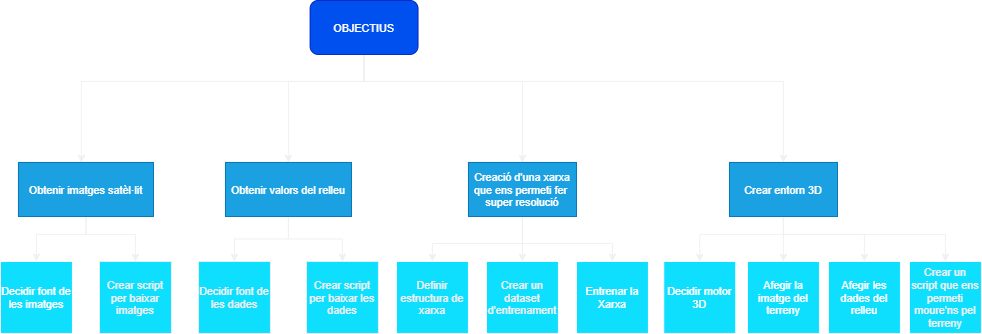
\includegraphics[scale = 0.5]{img/Objectius.png}
%\end{figure*}

\subsection{Metodologia}
Per tal de dur a terme aquest projecte d'una manera ordenada i rigurosa es farà ús de la metodología de \textit{Kanban}\cite{kanban}.
Aquesta metodología és considerada una metodologia \textit{"agile"} que ens obliga a portar un control precís del que s'ha fet, el que s'està fent i el que queda per fer mitjançant la repartició de la feina en tres columnes diferents que representen aquests estats.\\

Per tal de poder objectiu esmenat anteriorment, es farà ús d'una eina anomenada \textit{Trello}\cite{trello} i es crearàn tres columnes: una pels objectius complerts, una pels objectius en els que estèm treballant i una última pels objectius que encara no s'han fet.

\subsection{Planificació}

Per explicar la planificació del treball i alhora, per ajudar a l'organització d'aquest, s'ha realitzat un diagrama de Gantt.\cite{Gantt}
Aquest permet obtenir una vista general dels objectius programats, de manera que resulta molt senzill saber quines feines s'han de fer, quant temps s'ha de dedicar a cada tasca i, per tant, quan ha d'estar acabada cada una d'elles.\\

Aquest diagrama de Gantt es troba a l'apèndix, des de la [Figura \ref{fig:diagrama1}] fins la [Figura \ref{fig:diagrama5}]:\\


Per tal d'aconseguir els primers sub-objectius, s'hauràn de destinar un total de 44 hores [Figura \ref{fig:diagrama1}], la majoria d'elles destinades a llegir la documentació sobre la utilització de les APIs que seràn utilitzades, programant els scripts o documentant tota la feina feta.\\
D'altra banda, es pot veure que es destinen un baix nombre d'hores a prendre decisions un cop informats.\\


La [Figura \ref{fig:diagrama2}] de l'apèndix mostra el nombre d'hores dedicades al segon objectiu.\\
Com es pot observar, aquest ha augmentat fins a 80, destacant un altre cop el temps dedicat a crear l'script necessari per descarregar les imatges, el temps de consulta de l'API i la documentació del treball realitzat.\\
En aquesta figura es torna a identificar un baix número d'hores destinat a la presa de decisions, ja que es considera que si ja s'ha dedicat temps a la recerca d'informació, ja es té la base per poder prendre aquesta decisió d'una manera ràpida i correcta.\\


En la [Figura \ref{fig:diagrama3}] de l'apèndix, es pot observar com el numero d'hores creix fins a les 158 hores invertides. Això és degut a que aquest objectiu requereix tractar amb xarxes neuronals i, per tant, es precisa un major número d'hores per investigar quines hi ha, com funcionen i com podem crear-la.
A part, sol ser lent entrenar les xarxes i resoldre els errors que aquestes puguin tenir.
Finalment, al ser aquest un procés complicat, necessitarem bastant temps per documentar-ho tot d'una forma clara.\\


Com està representat en la [Figura \ref{fig:diagrama4}] de l'apèndix, s'ha incrementat la quantitat d'hores invertides fins a 232.
Això és degut a que, tot i estar tractant amb xarxes neuronals, com a l'objectiu anterior, és bastant possible que el tipus de xarxa que s'hagi d'utilitzar per cumplir aquest punt sigui diferent que la utilitzada anteriorment i, per tant, s'hagi de tornar a buscar informació  sobre el nou tipus de xarxa o, fins i tot, s'hagi d'utilitzar un altre entorn en el que la xarxa sigui més òptima.
Així doncs, es dedicarà bastant temps a documentar-se sobre els tipus de xarxes existents i a definir la nostra xarxa, així com a crear o obtenir un dataset, entrenar-la i mostrar els resultats obtinguts.
Afegidament, també s'haurà de documentar tot el procés.\\

Finalment, si ens fixem en la [Figura \ref{fig:diagrama5}] de l'apèndix, podem veure com el nostre projecte acaba ocupant 312 hores de treball. 
El motiu és que es dediquen moltes hores a la investigació dels diferents motors 3D per tal d'escollir el que interessa més per aquest treball. A part, també es dedica molt temps a investigar com funciona el motor escollit i a programar les diferents funcions que ens permetin afegir el relleu i les imatges a aquest, així com afegir la opció de que l'usuari es mogui pel terreny generat.\\


\section{Desenvolupament del treball}
\subsection{eleccio de la font de les imatges}
\begin{itemize}
\item Sentinel \cite{Sentinel}
\item NASA API \cite{NASA}
\item Google Earth API \cite{Earth}

\end{itemize}












\begin{thebibliography}{15}

\bibitem{kanban}
Laia Gilibets. (2020, November 11). Qué es la metodología Kanban y cómo utilizarla. Retrieved November 11, 2021, from Thinking for Innovation website: https://www.iebschool.com/blog/metodologia-kanban-agile-scrum/

\bibitem{trello}
Trello. (2019). Retrieved November 11, 2021, from Trello.com website: https://trello.com/

\bibitem{Gantt}
Waelput, B. (2021, August 18). ¿Qué es y para qué sirve un diagrama de Gantt? Retrieved October 6, 2021, from España website: https://www.teamleader.es/blog/diagrama-de-gantt

\bibitem{Sentinel}
Sentinel. (n.d.). SentinelHub API. SentinelHub API. Retrieved September 24, 2021, from https://www.sentinel-hub.com/develop/api/

\bibitem{NASA}
NASA. (n.d.). NASA Open APIs. NASA APIs. Retrieved September 24, 2021, from https://api.nasa.gov/

\bibitem{Earth}
Google. (n.d.). Google Earth Engine |. Google Developers. Retrieved September 24, 2021, from https://developers.google.com/earth-engine

\bibitem{icgc}
Codi obert i prototips. Institut Cartogràfic i Geològic de Catalunya. (2014). Retrieved October 2, 2021, from Icgc.cat website: https://www.icgc.cat/Aplicacions/Desenvolupadors/Codi-obert-i-prototips


\bibitem{Three}
Three.js – JavaScript 3D Library. (2021). Retrieved October 9, 2021, from Threejs.org website: https://threejs.org/

‌
\bibitem{Unity}
Unity Technologies. (2020). Unity - Unity. Retrieved October 9, 2021, from Unity website: https://unity.com/es

‌
\bibitem{unreal}
Unreal Engine | The most powerful real-time 3D creation tool. (2019). Retrieved October 9, 2021, from Unreal Engine website: https://www.unrealengine.com/en-US/?sessionInvalidated=true

‌
\bibitem{godot}
Godot Engine. (2021). Free and open source 2D and 3D game engine. Retrieved October 9, 2021, from Godot Engine website: https://godotengine.org/

‌\bibitem{Deep convolutional superResolution}
Song, Xibin, et al. Deep Depth Super-Resolution: Learning Depth Super-Resolution Using Deep Convolutional Neural Network. 20 Nov. 2016, pp. 366–382.

\bibitem{Desconvolutional}
Cao, Feilong, et al. “Deconvolutional Neural Network for Image Super-Resolution.” Neural Networks, vol. 132, Dec. 2020, pp. 394–404, 10.1016/j.neunet.2020.09.017. Accessed 7 Apr. 2021.

\bibitem{SRGAN}
Wenlong, Z., Yihao, L., Dong, C., \& Qiao, Y. (2021). RankSRGAN: Generative Adversarial Networks with Ranker for Image Super-Resolution. IEEE Transactions on Pattern Analysis and Machine Intelligence, 1–1. https://doi.org/10.1109/tpami.2021.3096327

\bibitem{iterative}
Saharia, C., Ho, J., Chan, W., Salimans, T., Fleet, D. J., \& Norouzi, M. (2021). Image Super-Resolution via Iterative Refinement. Retrieved October 10, 2021, from arXiv.org website: https://arxiv.org/abs/2104.07636

‌
‌
\end{thebibliography}

\begin{comment}
También he estado probando diferentes APIs para descargar las imágenes de forma automática (o para poder ir descargando según nos movemos si el área se tiene que ir generando según nos movemos por el mundo). 
Estuve mirando la de Sentinel, pero solo ofrece una prueba gratuïta de 10 dias.
También he encontrado alguna como la de Google Earth que nos permite obtener la elevación del terreno con solo dar las coordenadas, lo cual nos podría ser útil para ir generando el relieve del terreno sobre la marcha.
También existe la de la NASA, aunque es bastante lenta a la hora de ofrecernos las imágenes (y en muchas hay nubes).

En general todas las APIs tardan unos segundos en devolver la imagen lo que puede darnos problemas 
\end{comment}

\clearpage
\onecolumn
\begin{appendix}
\appendix
\section{Apèndix}

\begin{figure}[H]
\centering
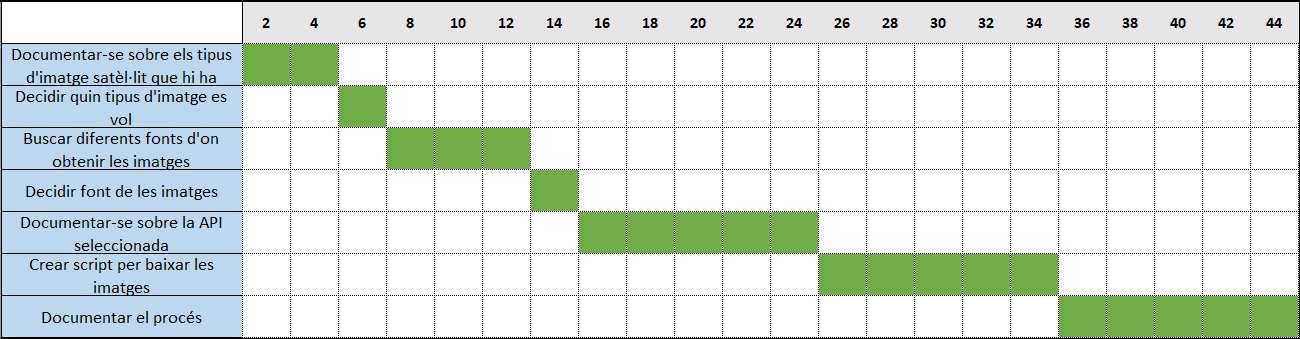
\includegraphics[width=\textwidth]{img/diagrama1.png}
\caption{Diagrama de Gantt del primer objetiu}
\label{fig:diagrama1}
\end{figure}

 \begin{figure}[H]
\centering
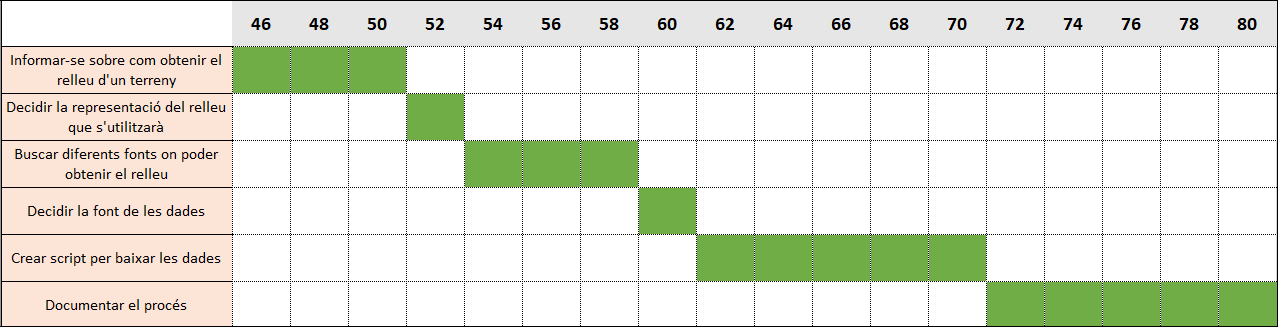
\includegraphics[width=\textwidth]{img/diagrama2.png}
\caption{Diagrama de Gantt del segon objetiu}
\label{fig:diagrama2}
\end{figure}

\begin{figure}[H]
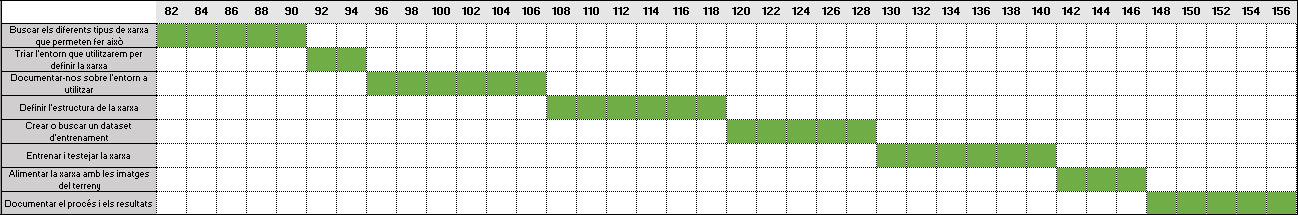
\includegraphics[width=\textwidth]{img/diagrama3.png}
\caption{Diagrama de Gantt del tercer objetiu}
\label{fig:diagrama3}
\end{figure}

 \begin{figure}[H]
\centering
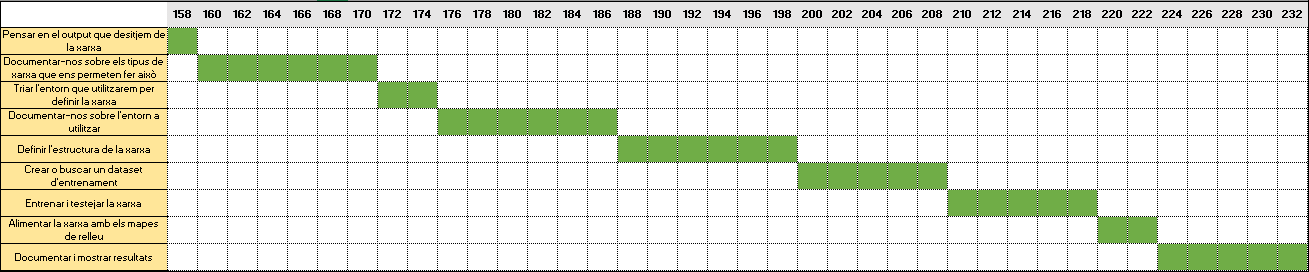
\includegraphics[width=\textwidth]{img/diagrama4.png}
\caption{Diagrama de Gantt del quart objetiu}
\label{fig:diagrama4}
\end{figure}

 \begin{figure}[H]
\centering
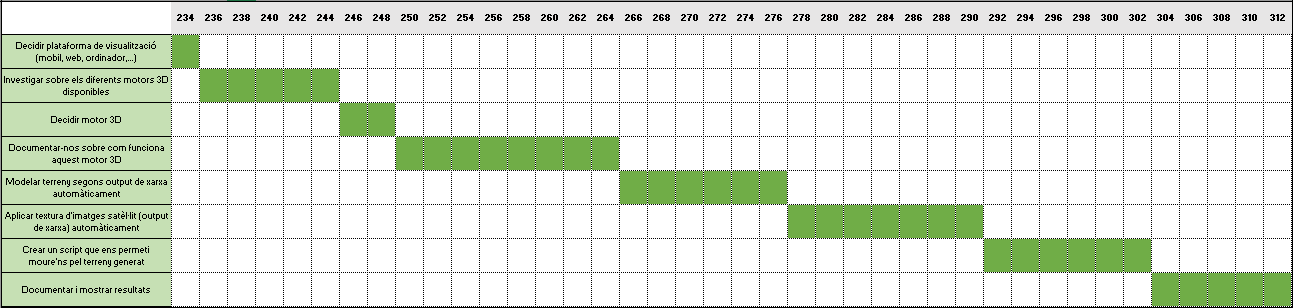
\includegraphics[width=\textwidth]{img/diagrama5.png}
\caption{Diagrama de Gantt del cinquè objetiu}
\label{fig:diagrama5}
\end{figure}
\end{appendix}
\end{document}

